\chapter{Aplicación web VeriSon}
\label{cap:aplicacion-web}

\section{Objetivo y alcance}

Como prueba de concepto, se ha desarrollado VeriSon, una aplicación web que permite analizar canciones y presentar una estimación sobre el posible origen del contenido, distinguiendo entre origen humano y generación mediante IA. La aplicación integra el enfoque seleccionado en el capítulo~\ref{cap:validacion}: MFCC + \textit{StandardScaler} + SVM RBF.

Su funcionamiento es el siguiente: el usuario proporciona un archivo de audio, que se somete a las etapas de preprocesamiento, extracción de características y clasificación descritas en este capítulo. Tras el análisis, la interfaz presenta una estimación cualitativa sobre su posible origen. De este modo, la aplicación conecta el trabajo experimental con una solución software utilizable.

\section{Arquitectura y tecnologías}

VeriSon adopta una arquitectura cliente-servidor formada por dos componentes independientes: una aplicación web de una sola página que organiza la interacción con el usuario y un servicio backend que encapsula la API y el pipeline de inferencia. El archivo de audio se envía al backend mediante una petición HTTP \textit{multipart/form-data}, mientras que el resultado del análisis se devuelve en una respuesta JSON. Esta separación desacopla la interfaz de la lógica de análisis y permite desplegar ambos componentes de forma independiente.

\begin{figure}[htbp]
    \centering
    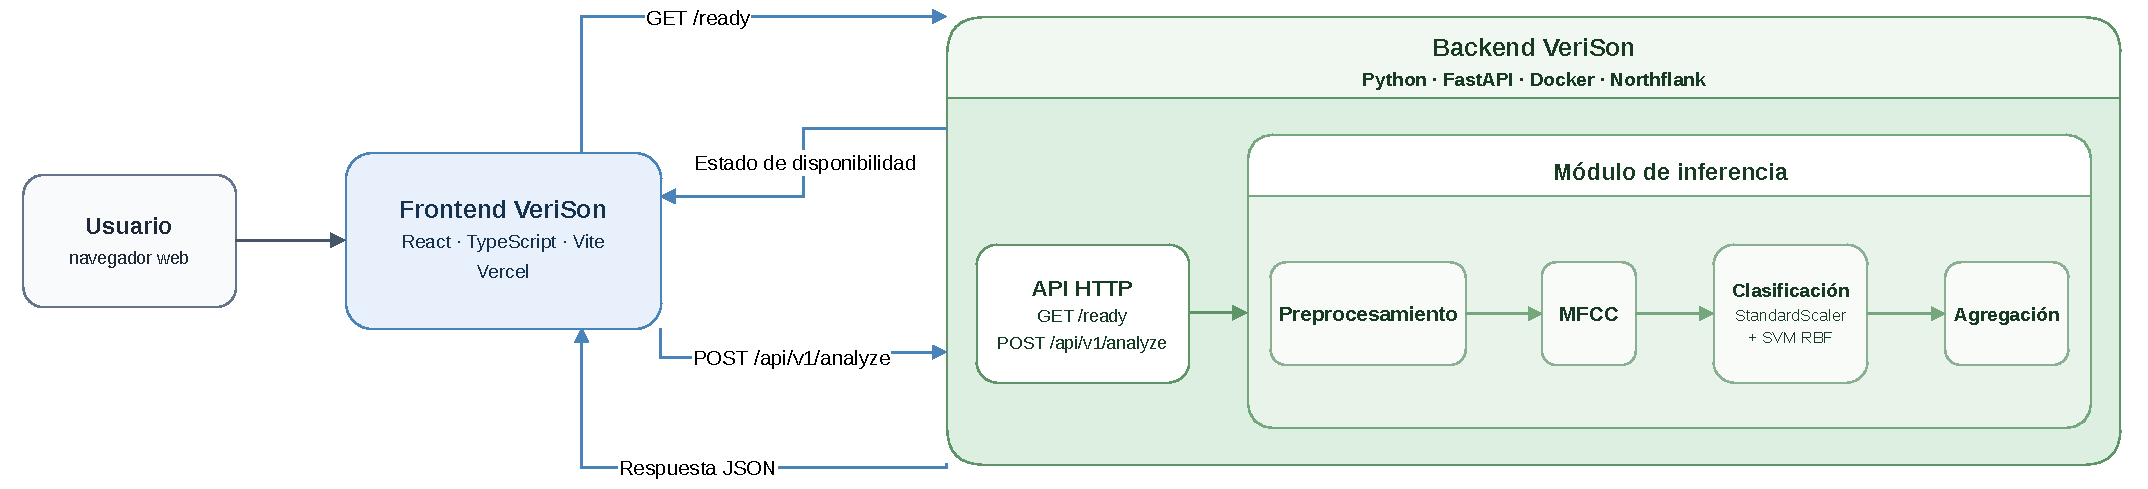
\includegraphics[width=\textwidth]{fig/arquitectura_verison.pdf}
    \caption{Arquitectura general de la aplicación web VeriSon.}
    \label{fig:arquitectura-verison}
\end{figure}

El frontend se implementa con React, TypeScript y Vite. React organiza la interfaz y los estados de interacción; TypeScript aporta tipado estático al cliente y a las estructuras utilizadas en la comunicación con la API, y Vite proporciona el entorno de desarrollo y construcción. El frontend se despliega en Vercel, elegido por la facilidad de despliegue de aplicaciones construidas con Vite y por disponer de una opción sin coste adecuada para las necesidades de este componente.

Dado que el pipeline de procesamiento y el modelo seleccionado se ejecutan en Python, el backend se implementa en el mismo lenguaje, lo que permite integrar directamente la lógica de inferencia. FastAPI se utiliza como framework para exponer esta funcionalidad mediante una API HTTP y Docker permite definir y reproducir el entorno del backend junto con sus dependencias. Para el despliegue del servicio contenerizado se seleccionó Northflank, al ofrecer dentro del plan utilizado recursos suficientes para ejecutar el backend sin coste para el proyecto.

El código de la aplicación web se mantiene en el mismo repositorio GitHub que el resto del proyecto y la experimentación, lo que centraliza el versionado y su evolución conjunta. Por este motivo, se utiliza GitHub Actions para la integración continua, aprovechando su integración directa con el repositorio, las \textit{pull requests} y los \textit{checks}.

\section{Backend y flujo de inferencia}

\subsection{API y validación de entrada}

Al iniciar el servicio, la función de ciclo de vida crea una única instancia del servicio de inferencia, carga el artefacto del modelo y verifica su compatibilidad con la configuración esperada. Si estas operaciones concluyen correctamente, el modelo queda disponible para las solicitudes posteriores; si fallan, el servicio conserva un estado degradado y comunica que el análisis no está disponible. Este comportamiento evita cargar el modelo para cada petición y permite diferenciar la disponibilidad de la API de la disponibilidad efectiva de la inferencia.

La tabla~\ref{tab:endpoints-verison} resume los puntos de acceso públicos de la API.

\begin{table}[htbp]
    \centering
    \caption{Puntos de acceso principales de la API de VeriSon.}
    \label{tab:endpoints-verison}
    \begin{tabular}{p{0.25\textwidth}p{0.18\textwidth}p{0.47\textwidth}}
        \toprule
        \textbf{Ruta} & \textbf{Método} & \textbf{Finalidad} \\
        \midrule
        /health & GET & Informa del estado general del servicio y de la carga del modelo. \\
        /ready & GET & Indica si el servicio está preparado para aceptar análisis. \\
        /api/v1/model & GET & Devuelve la información disponible sobre el artefacto del modelo cargado. \\
        /api/v1/analyze & POST & Recibe un archivo de audio y devuelve el resultado de la inferencia. \\
        \bottomrule
    \end{tabular}
\end{table}

Por su parte, \textit{GET /ready} comprueba específicamente si el servicio está preparado para aceptar análisis. Durante la inicialización o el \textit{warm-up}, la API puede ser accesible y responder a la comprobación general, pero este endpoint mantiene el estado de no disponibilidad para análisis hasta que finaliza dicha preparación.

La solicitud \textit{POST /api/v1/analyze} recibe el archivo mediante \textit{multipart/form-data}. Se aceptan archivos WAV y MP3 y, antes de iniciar la extracción de características y la clasificación, el backend realiza las siguientes validaciones:

\begin{itemize}
    \item Extensión y, cuando está disponible, tipo MIME.
    \item Contenido no vacío.
    \item Tamaño máximo, configurable y de 64 MiB por defecto.
    \item Duración máxima, configurable y de 300~s por defecto.
    \item Posibilidad de decodificar correctamente el audio.
\end{itemize}

Cuando alguna validación falla, la API devuelve una respuesta controlada y diferenciada según la causa. También existen respuestas controladas cuando el modelo no está disponible o se produce un fallo durante la inferencia, lo que permite al frontend traducirlas a mensajes adecuados.

Para procesar la carga, el backend copia el contenido recibido en un archivo temporal. Dicho archivo se utiliza durante la decodificación y se elimina tanto tras una inferencia correcta como cuando se produce una excepción, de modo que no se acumulan archivos de usuario en el servicio.

\subsection{Preprocesamiento e inferencia}

El archivo de audio se recorre de forma secuencial en fragmentos de hasta 10~s. Cada bloque se convierte a mono cuando procede y se remuestrea a 16~kHz; únicamente el último se completa mediante \textit{padding} cuando no alcanza la duración objetivo. Para cada fragmento se conserva además su duración original, utilizada posteriormente en la agregación de las decisiones parciales.

El tratamiento temporal difiere del empleado en el baseline experimental. Cuando un audio superaba los 10~s, el baseline seleccionaba una única ventana de 10~s de máxima energía. VeriSon, en cambio, analiza todos los bloques obtenidos mediante la segmentación anterior para cubrir el archivo proporcionado por el usuario.

Para cada fragmento se calculan 20 coeficientes MFCC. La media y la desviación típica temporal de cada coeficiente forman un vector de 40 características, que se transforma con el \textit{StandardScaler} y se clasifica mediante la SVM con núcleo RBF. El clasificador produce una puntuación de decisión, cuyo signo se compara con el umbral global cero.

\subsection{Agregación y respuesta}

Para obtener una única estimación a nivel de archivo, las puntuaciones de los fragmentos se combinan mediante una media ponderada por su duración original. Si $s_i$ representa la puntuación del fragmento $i$ y $d_i$ su duración antes de aplicar el \textit{padding}, de forma que el relleno del último fragmento no incremente artificialmente su peso, la puntuación global se calcula como:

\[
    S = \frac{\sum_{i=1}^{n} d_i s_i}{\sum_{i=1}^{n} d_i}.
\]

El signo de $S$ se compara con el mismo umbral global cero utilizado en cada fragmento para obtener la clase final. A partir de este resultado, la respuesta JSON agrupa la siguiente información:

\begin{itemize}
    \item el resultado global y su puntuación.
    \item la información del audio analizado, como la duración y el número de fragmentos.
    \item los resultados individuales de los fragmentos.
    \item los tiempos e información técnica del modelo.
\end{itemize}

Esta estructura permite al frontend mostrar la información necesaria para la interfaz, mientras que la API mantiene el detalle técnico del análisis.

\section{Frontend e interacción con el usuario}

\subsection{Flujo de interacción}

La interfaz guía al usuario desde la selección del archivo hasta la visualización del resultado. Antes de iniciar el análisis, valida localmente que la extensión corresponda a WAV o MP3. El flujo distingue los estados \textit{idle}, \textit{selected}, \textit{preparing}, \textit{analyzing}, \textit{success} y \textit{error}, e impide solicitudes duplicadas mientras existe una operación activa. El usuario puede volver a seleccionar otro archivo mediante el reinicio del flujo; si existe una petición activa, esta se cancela al reiniciarlo o cuando el componente se desmonta.

\begin{figure}[H]
    \centering
    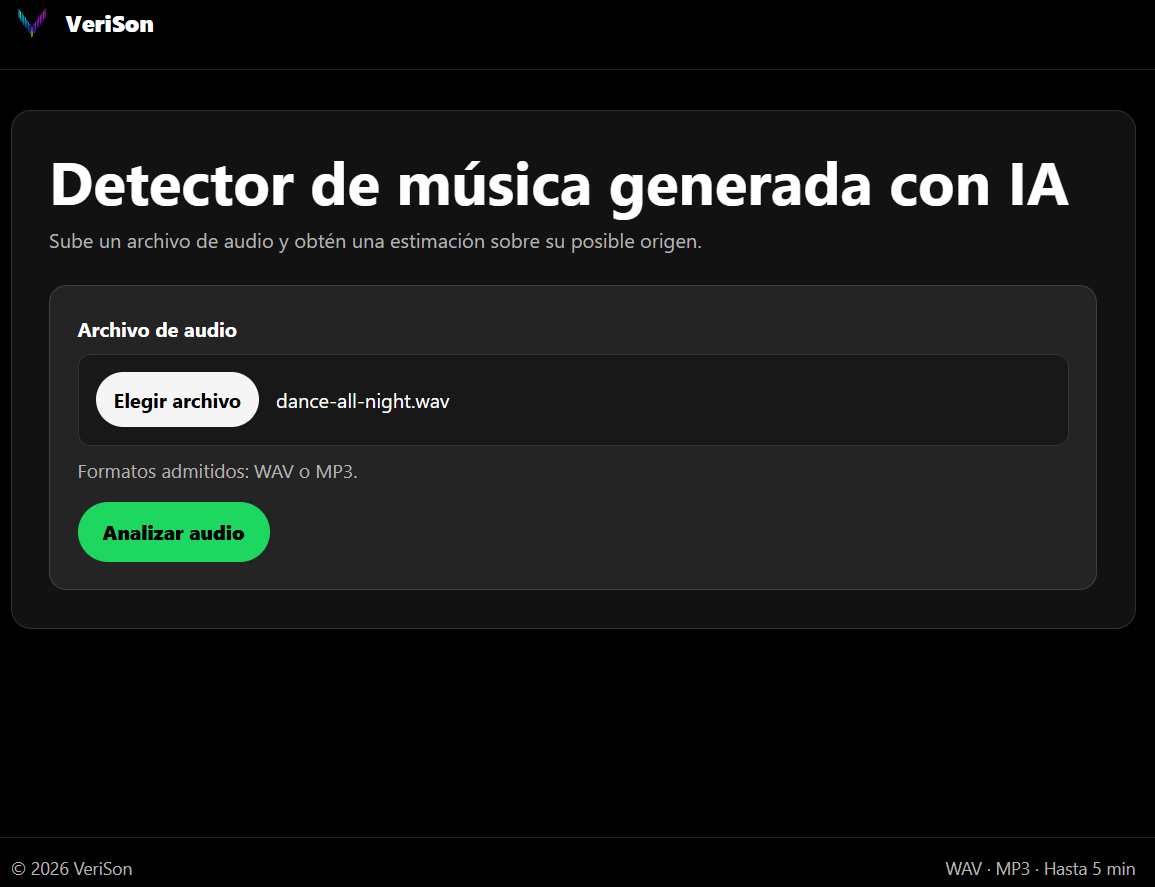
\includegraphics[width=0.82\textwidth]{fig/verison_home.png}
    \caption{Estado de VeriSon tras seleccionar un archivo WAV válido.}
    \label{fig:validacion-inicio}
\end{figure}

\subsection{Comunicación con el backend}

La URL pública del backend se configura mediante una variable de entorno del frontend. Antes de enviar el archivo, el cliente consulta \textit{GET /ready}. Las respuestas transitorias de disponibilidad se reintentan durante un presupuesto total de 15~s, con sondeos cada 5~s y un límite individual de 5~s por consulta. Cuando el backend informa que está preparado, el cliente envía \textit{POST /api/v1/analyze} con el audio en \textit{multipart/form-data}. La solicitud de análisis dispone de un \textit{timeout} de 180~s y no se reintenta automáticamente, para evitar duplicar la operación ante una respuesta incierta.

\subsection{Presentación del resultado}

Tras una respuesta correcta, la interfaz muestra el nombre del archivo, la etiqueta \textit{Posible generación con IA} o \textit{Posible origen humano} y un mensaje explicativo asociado al resultado. Ante un error, interpreta la respuesta técnica del backend, la transforma en un mensaje comprensible, refleja el estado \textit{error} y permite volver al flujo normal. También gestiona errores propios del cliente, como problemas de red o \textit{timeout}.

\begin{figure}[H]
    \centering
    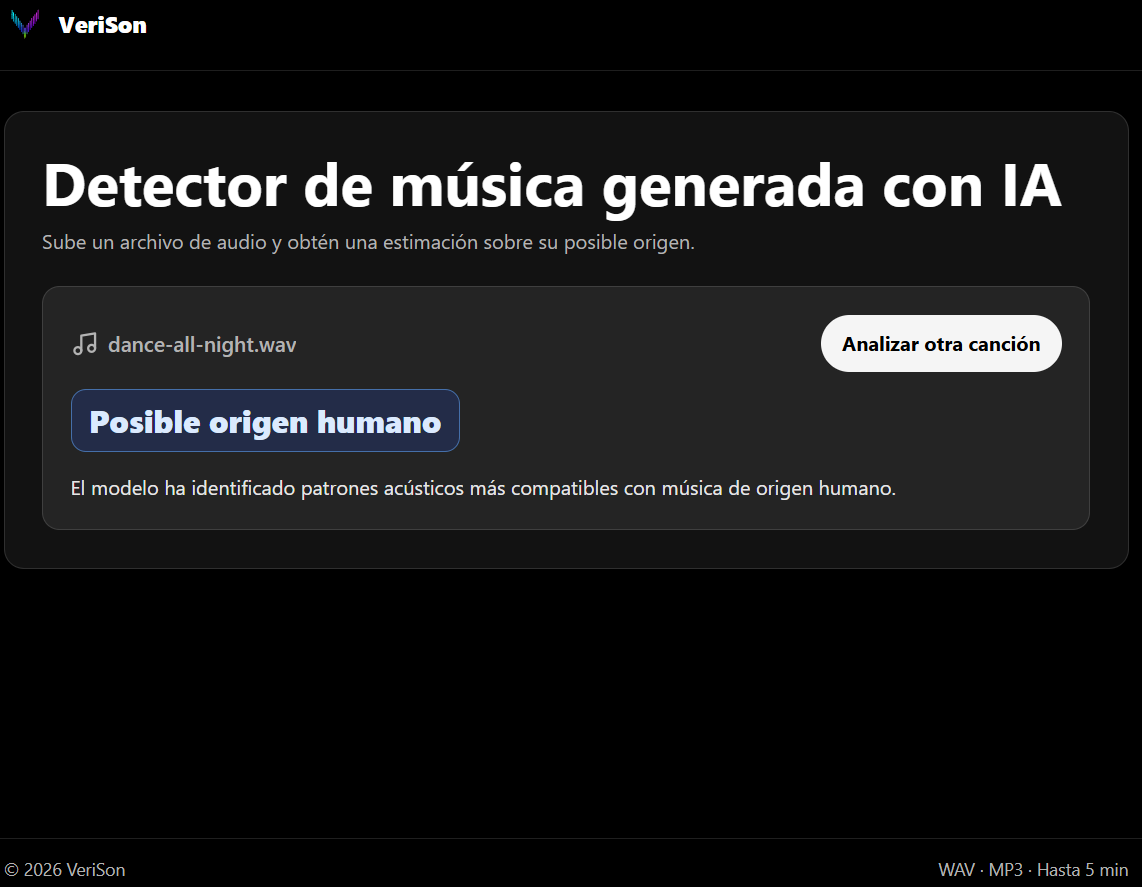
\includegraphics[width=0.82\textwidth]{fig/verison_wav_human.png}
    \caption{Resultado de un análisis con un archivo WAV.}
    \label{fig:validacion-wav}
\end{figure}

\begin{figure}[H]
    \centering
    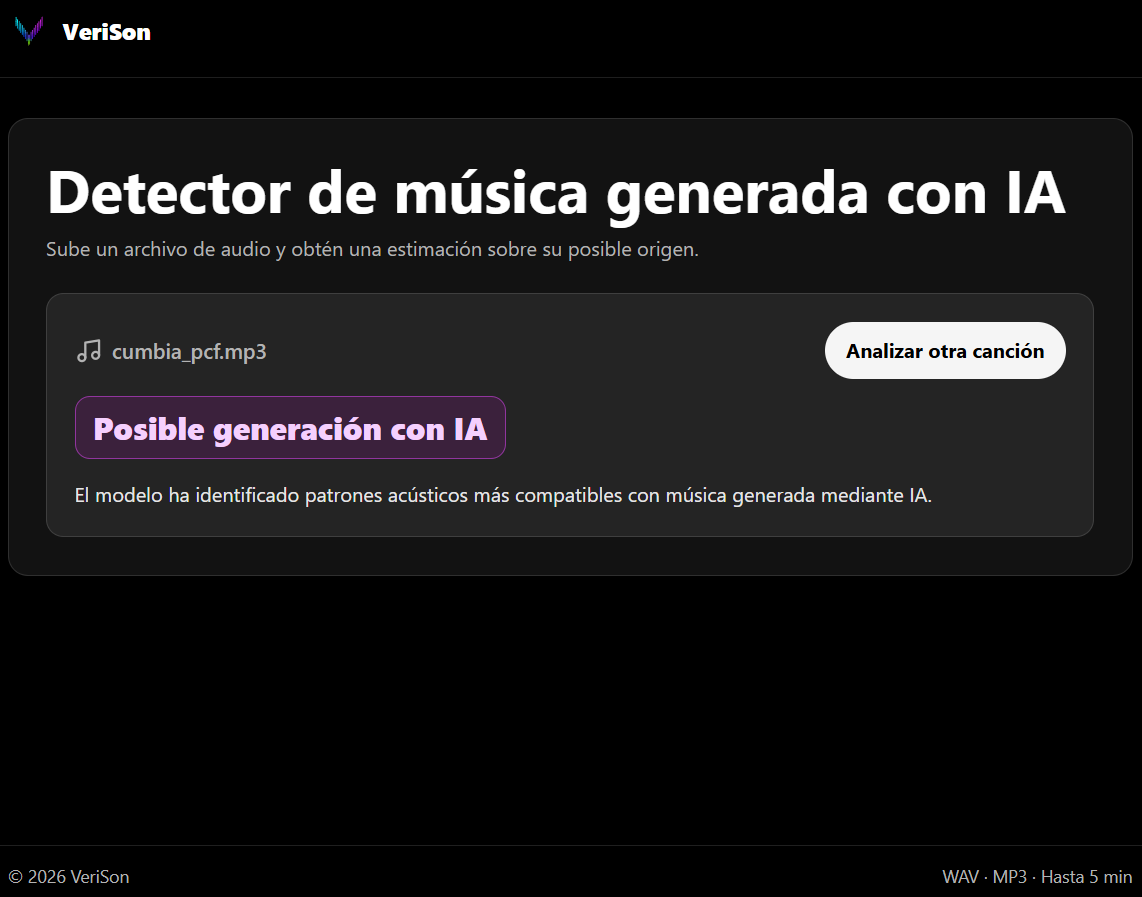
\includegraphics[width=0.82\textwidth]{fig/verison_ai.png}
    \caption{Resultado de un análisis con un archivo MP3.}
    \label{fig:validacion-mp3}
\end{figure}

\begin{figure}[H]
    \centering
    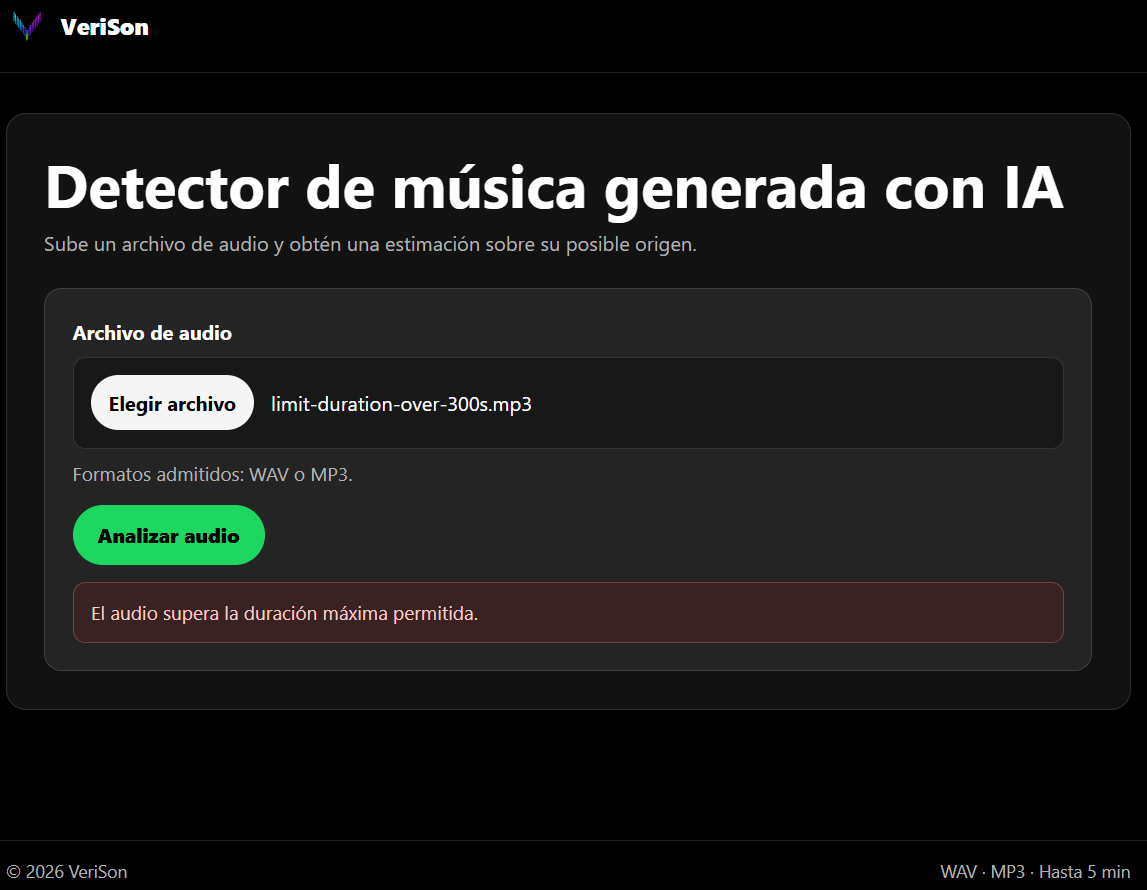
\includegraphics[width=0.82\textwidth]{fig/verison_limit_duration.png}
    \caption{Mensaje mostrado tras rechazar un audio que supera la duración máxima permitida.}
    \label{fig:error-backend-duracion}
\end{figure}

\section{Despliegue e integración continua}

\subsection{Despliegue}

El frontend se despliega en Vercel y el backend, junto con el artefacto del modelo, se ejecuta en Northflank mediante una imagen Docker. La URL pública del backend se proporciona al frontend mediante su configuración de entorno, y la política CORS del backend autoriza el origen del cliente desplegado. La imagen Docker instala las dependencias de Python, incorpora el código del servicio y el artefacto necesario para la inferencia, e inicia el servicio FastAPI mediante Uvicorn en el puerto indicado por el entorno.

El servicio desplegado en Northflank utiliza una única instancia y dispone de 0,2 vCPU compartida, 512 MiB de memoria y 1 GiB de almacenamiento efímero. Debido al límite de memoria disponible, el procesamiento del audio se reorganizó para reducir la cantidad de datos mantenidos simultáneamente. Para ello, el archivo se abre una sola vez y se recorre de forma secuencial, procesando cada fragmento y transformándolo inmediatamente en su vector de 40 características. Hasta la clasificación solo se conservan estos vectores y sus metadatos, evitando mantener en memoria al mismo tiempo el audio completo y las señales intermedias de todos los fragmentos.

También se incorporó un \textit{warm-up} durante el arranque para evitar que el coste de inicialización recaiga sobre el primer análisis. Tras cargar el artefacto del modelo, y con la configuración de despliegue activada, el servicio ejecuta en segundo plano un remuestreo sintético de 1~s desde 48~kHz hasta 16~kHz y, si este concluye correctamente, una extracción MFCC sobre una señal sintética de la longitud objetivo. Ambas operaciones utilizan las mismas funciones que el análisis. Mientras este proceso está pendiente, \textit{GET /ready} no declara preparado el servicio y el frontend espera antes de enviar un archivo real. Cuando las dos operaciones finalizan correctamente, el estado de preparación pasa a disponible; si alguna falla, permanece no disponible para análisis.

En el momento del depósito de este TFM, la prueba de concepto web se encuentra accesible públicamente en \url{https://verison-app.vercel.app}. Al depender de servicios externos de despliegue, no se garantiza la disponibilidad indefinida de esta instancia.

\subsection{Integración continua}

El workflow de GitHub Actions se ejecuta ante cada \textit{pull request} a \textit{main} y cada \textit{push} a \textit{main}. La protección de esta rama requiere una \textit{pull request} y que los tres \textit{checks} definidos a continuación finalicen correctamente antes del \textit{merge}:

\begin{itemize}
    \item \textbf{Backend}: utiliza Python 3.11.9, instala las dependencias y ejecuta la suite implementada con \textit{pytest}, que cubre el procesamiento e inferencia, las validaciones de la API y la inicialización y disponibilidad del servicio.

    \item \textbf{Frontend}: utiliza Node 20.19.0, instala las dependencias y ejecuta \textit{npm run check}, un comando del proyecto que agrupa el \textit{lint}, la comprobación del \textit{build} y las pruebas automatizadas con \textit{Vitest}. Estas verifican el comportamiento de la interfaz, la validación de formatos, la comunicación con la API y la gestión de estados y errores.

    \item \textbf{Docker}: comprueba que la imagen del backend puede construirse correctamente mediante el Dockerfile de despliegue.
\end{itemize}

\begin{figure}[H]
    \centering
    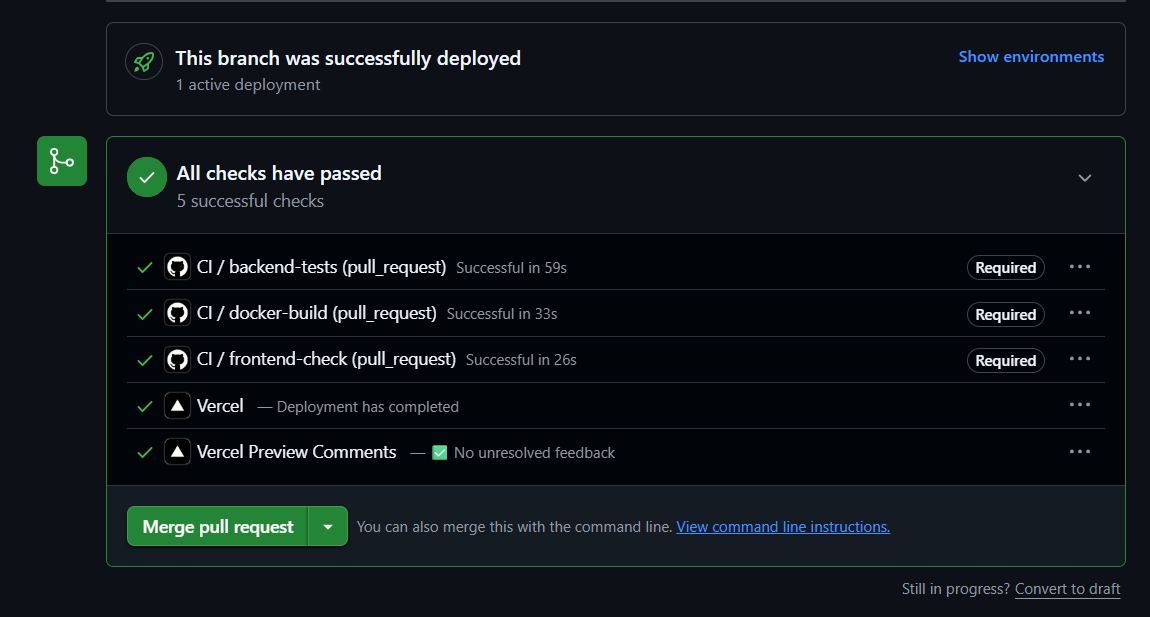
\includegraphics[width=0.82\textwidth]{fig/allchecks.png}
    \caption{Checks obligatorios de integración continua superados en una \textit{pull request}.}
    \label{fig:ci-checks}
\end{figure}

GitHub Actions se utiliza exclusivamente como mecanismo de integración continua: verifica el código, las pruebas y el empaquetado antes de integrar cambios en \textit{main}, pero no publica la imagen Docker ni realiza los despliegues en Northflank o Vercel. Por tanto, no constituye un pipeline completo de CI/CD.
